\documentclass[border=6pt]{standalone}
\usepackage{amsmath}
\usepackage{tikz}
\usetikzlibrary{arrows.meta,positioning,shapes.geometric}

\begin{document}
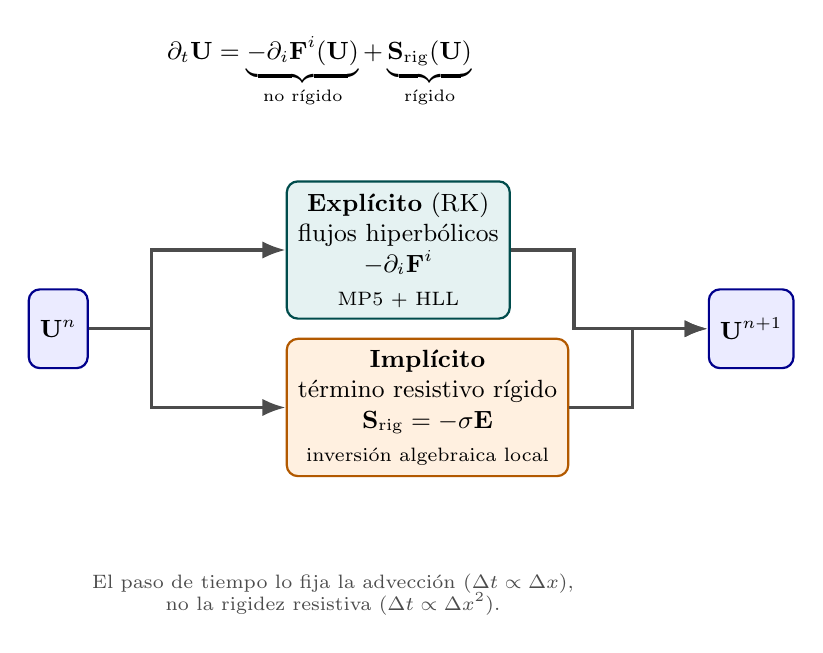
\begin{tikzpicture}[>=Latex,node distance=8mm,
  box/.style={draw,thick,rounded corners,align=center,minimum height=10mm,inner sep=4pt,font=\small},
  exp/.style={box,fill=teal!10,draw=teal!60!black},
  imp/.style={box,fill=orange!12,draw=orange!70!black},
  st/.style={box,fill=blue!8,draw=blue!55!black},
  ar/.style={->,very thick,black!70}]

% Estado inicial
\node[st] (un) {$\mathbf U^{n}$};

% Parte explícita (Mover un poco a la derecha si es necesario para dar aire)
\node[exp,right=25mm of un,yshift=10mm] (ex)
  {\textbf{Expl\'icito} (RK)\\ flujos hiperb\'olicos\\ $-\partial_i\mathbf F^{i}$\\[1pt]\scriptsize MP5 $+$ HLL};

% Parte implícita
\node[imp,right=25mm of un,yshift=-10mm] (im)
  {\textbf{Impl\'icito}\\ t\'ermino resistivo r\'igido\\ $\mathbf S_{\rm rig}=-\sigma\mathbf E$\\[1pt]\scriptsize inversi\'on algebraica local};

% Ecuación de división: Ahora posicionada de forma absoluta sobre el centro del bloque explícito
% Se incrementó la distancia vertical (above=8mm) para dar espacio a los \underbrace
\node[font=\small,align=center,above=8mm of ex.north,xshift=-10mm] (split)
  {$\partial_t\mathbf U=\underbrace{-\partial_i\mathbf F^{i}(\mathbf U)}_{\text{no r\'igido}}+\underbrace{\mathbf S_{\rm rig}(\mathbf U)}_{\text{r\'igido}}$};

% Estado final
\node[st,right=25mm of ex,yshift=-10mm] (un1) {$\mathbf U^{n+1}$};

% Conexiones con quiebres limpios empleando la coordenada x del punto medio
\draw[ar] (un.east) -- ++(0.8,0) |- (ex.west);
\draw[ar] (un.east) -- ++(0.8,0) |- (im.west);
\draw[ar] (ex.east) -- ++(0.8,0) |- (un1.west);
\draw[ar] (im.east) -- ++(0.8,0) |- (un1.west);

\node[font=\scriptsize,black!70,below=11mm of im.south,xshift=-12mm,align=center]
  {El paso de tiempo lo fija la advecci\'on ($\Delta t\propto\Delta x$),\\ no la rigidez resistiva ($\Delta t\propto\Delta x^{2}$).};

\end{tikzpicture}
\end{document}